\documentclass[12pt, oneside]{article}
\usepackage[letterpaper,scale=0.85, centering]{geometry}
\usepackage{amssymb,amsmath}
\usepackage{currfile,xstring,hyperref}
\usepackage[labelformat=empty]{caption}
\usepackage[dvipsnames,table]{xcolor}
\usepackage{multicol}
\usepackage{listings}
\usepackage{graphicx}
\graphicspath{ {./images/} }

% NOTE(joe): This environment is credit @pnpo (https://tex.stackexchange.com/a/218450)
\lstnewenvironment{algorithm}[1][] %defines the algorithm listing environment
{   
    \lstset{ %this is the stype
        mathescape=true,
        frame=tB,
        numbers=left, 
        numberstyle=\tiny,
        basicstyle=\rmfamily\scriptsize, 
        keywordstyle=\color{black}\bfseries,
        keywords={,procedure, div, for, to, input, output, return, datatype, function, in, if, else, foreach, while, begin, end, }
        numbers=left,
        xleftmargin=.04\textwidth,
        #1
    }
}
{}

\lstnewenvironment{java}[1][]
{   
    \lstset{
        language=java,
        mathescape=true,
        frame=tB,
        numbers=left, 
        numberstyle=\tiny,
        basicstyle=\ttfamily\scriptsize, 
        keywordstyle=\color{black}\bfseries,
        keywords={, int, double, for, return, if, else, while, }
        numbers=left,
        xleftmargin=.04\textwidth,
        #1
    }
}
{}

\setlength{\parindent}{0em}
\setlength{\parskip}{0.5em}

\title{\bf CSE 103 \\[2ex]
       \Large Homework \#6\\ Fall 2019}
\begin{document}
\date{\textbf{Due}: Monday, November 11, 2019 at 11:00PM on Gradescope}
\maketitle
%$\\[-50pt]$

\section{Directions}
You may work with one other student. If working with a partner,
\textbf{submit only one submission per pair} : one partner uploads the submission and adds the other partner to the Gradescope submission. You can post public questions about the assignment to Piazza, discuss the questions and their answers with at most one other student, and ask questions in office hours

Your answers have to be typeset, not handwritten. This is for two
reasons: (a) to reduce ambiguity of the answers, and (b) to be kind to
the TA's eyesight. We recommend you use latex, but you can also use
word-processors that support mathematical formulas. More directions
are available here: {\tt https://tinyurl.com/y2gv9bn9}.

You will submit this assignment via Gradescope
(\url{https://www.gradescope.com}) in the assignment called ``Homework
3''. You can submit each question as many times as you like. You should solve the problems and ask questions about them offline first, then try submitting once you are confident in your answers. 

\textbf{No late submissions are accepted.}


  \newpage
\section{Problems}
\begin{enumerate}

\item (15 points) Suppose that a study were done on married couple in a small town. We learned that one person in each couple is always exactly $7\%$ shorter than their partner. What would the correlation between the heights of the married couple be?

\newpage
\item (30 points + Additional 5 points for providing legible and organized answers) In each of the three questions below, compute the mean and std of x and of y and the correlation of x and y

Using the grid provided, create a plot of the means, std  and SD lines as shown in the example.


\begin{table}[h!]
  \begin{center}
    \caption{\textbf{Table a:}}
    \label{tab:table1}
    \begin{tabular}{l|S}
      \textbf{$x$} & \textbf{$y$} \\
     
      \hline
      6 &  0\\
 5 &  2\\
 5 &  1\\
 2 &  4\\
-2 &  7\\
 7 &  0\\
 7 &  2\\
 1 &  3\\

    \end{tabular}
  
  \end{center}
 
\end{table}

\begin{center}
     
  
\includegraphics{grid.png}
\end{center}

\newpage

\begin{table}[h!]
  \begin{center}
    \caption{\textbf{Table b:}}
    \label{tab:table1}
    \begin{tabular}{l|S}
      \textbf{$x$} & \textbf{$y$} \\
     
      \hline
      -2 &  4\\
-3 &  7\\
 0 & -1\\
-3 &  5\\
-3 & -3\\
-2 &  4\\
-2 & -3\\
-1 & -2\\
    \end{tabular}
  
  \end{center}
 
\end{table}

\begin{center}
     
  
\includegraphics{grid.png}
\end{center}

\newpage

\begin{table}[h!]
  \begin{center}
    \caption{\textbf{Table c:}}
    \label{tab:table1}
    \begin{tabular}{l|S}
      \textbf{$x$} & \textbf{$y$} \\
     
      \hline
      5 &  7\\
 5 & -2\\
 1 &  2\\
 1 &  1\\
 0 &  2\\
 3 &  5\\
 1 &  2\\
 3 & -6\\
-1 & -4\\
-6 &  0\\
-4 & -1\\
-3 &  5\\

    \end{tabular}
  
  \end{center}
 
\end{table}

\begin{center}
     
  
\includegraphics{grid.png}
\end{center}

\newpage

\begin{table}[h!]
  \begin{center}
    \caption{\textbf{Example:}}
    \label{tab:table1}
    \begin{tabular}{l|S}
      \textbf{$x$} & \textbf{$y$} \\
     
      \hline
      5 &  3\\
 8 &  4\\
 7 &  4\\
 3 &  2\\
2 &  1\\
 5 &  3\\
 2 &  1\\
 8 &  4\\

    \end{tabular}
  
  \end{center}
 
\end{table}



     \textbf{Expected answer:}
     
     
\begin{center}
  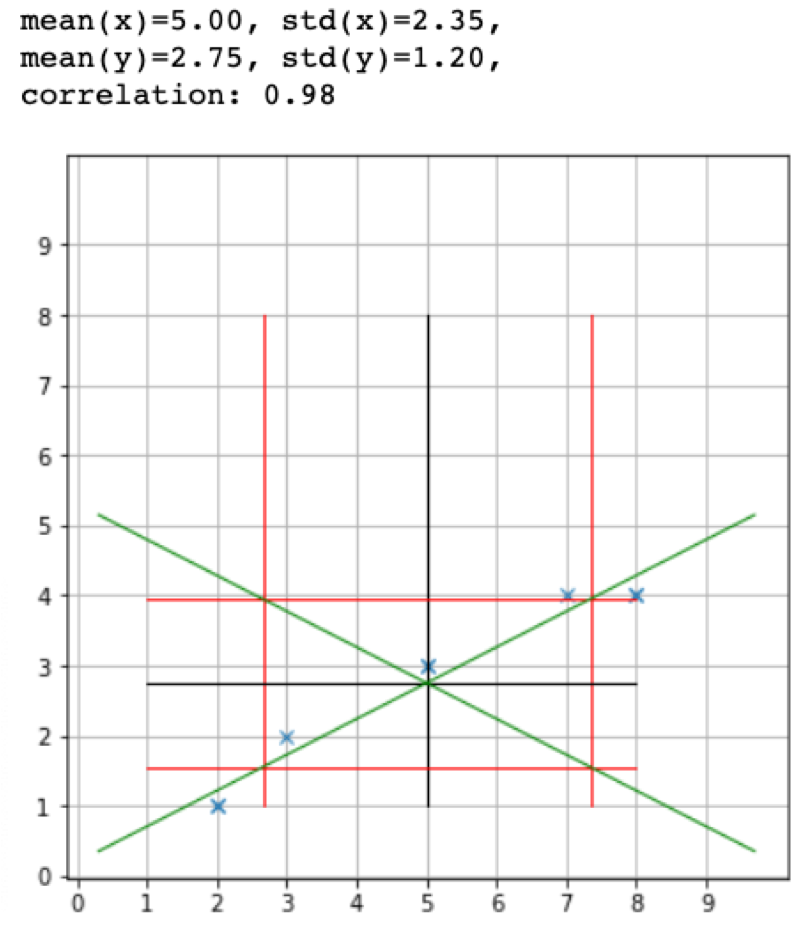
\includegraphics{expected.png}
\end{center}

\newpage



\item (20 points) A study was conducted on identical twins. The IQs of the twins were obtained:

Older twin: average IQ$= 100$, SD $= 15$

Younger twin: average IQ$=100$, SD $= 15$

$r=0.6$

One of the following is a scatter diagram for the data. Which one? Explain briefly why the others are rejected.
\begin{center}
  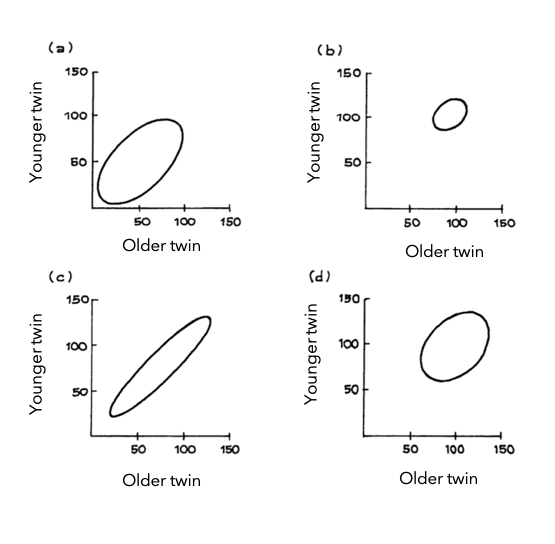
\includegraphics[scale=0.5]{problem3.png}
  
\end{center}

\newpage



\item (30 points) The figure below has six scatter diagrams for hypothetical data. The correlation coefficients, in scrambled order, are:
$$-0.85 \quad -0.38\quad-1.00\quad0.06\quad0.97\quad0.62$$

Match the scatter diagrams with the correlation coefficients.
\begin{center}
  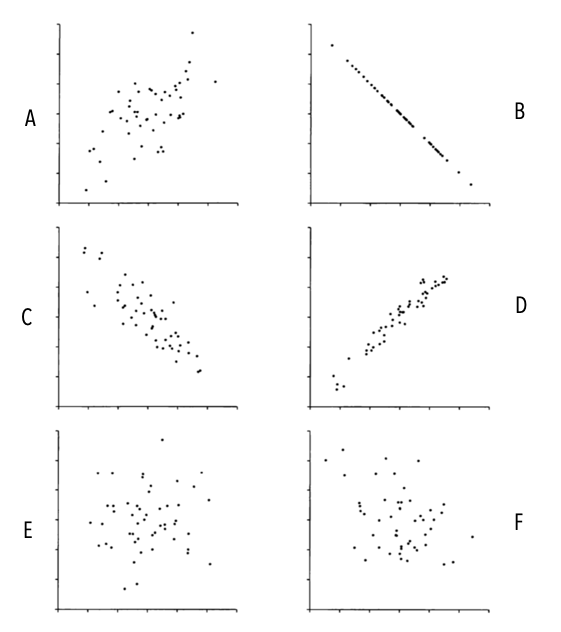
\includegraphics[scale=0.5]{problem4.png}
\end{center}
\end{enumerate}
\end{document}
